%TC第29.1节练习 4、5
%TC第29.2节练习 2、4、6
%TC第29.3节练习 5
%TC第29.4节练习 2
%%%%%%%%%%%%%%%%%%%%%%%%%%%%%%%%%%%%%%%%%%%%%%%%%%%%%%%%%%%%%%%%
\documentclass[11pt, a4paper, UTF8]{ctexart}
%%%%%%%%%%%%%%%%%%%%%%%%%%%%%%%%%%%
% File: preamble.tex
%%%%%%%%%%%%%%%%%%%%%%%%%%%%%%%%%%%

\usepackage[top = 1.5cm]{geometry}

% Set fonts commands
\newcommand{\song}{\CJKfamily{song}} 
\newcommand{\hei}{\CJKfamily{hei}} 
\newcommand{\kai}{\CJKfamily{kai}} 
\newcommand{\fs}{\CJKfamily{fs}}

\newcommand{\me}[2]{\author{{\bfseries 姓名:}\underline{#1}\hspace{2em}{\bfseries 学号:}\underline{#2}}}

% Always keep this.
\newcommand{\noplagiarism}{
  \begin{center}
    \fbox{\begin{tabular}{@{}c@{}}
      请独立完成作业,不得抄袭。\\
      若得到他人帮助, 请致谢。\\
      若参考了其它资料,请给出引用。\\
      鼓励讨论,但需独立书写解题过程。
    \end{tabular}}
  \end{center}
}

% Each hw consists of three parts:
% (1) this homework
\newcommand{\beginthishw}{\part{作业}}
% (2) corrections (Optional)
\newcommand{\begincorrection}{\part{订正}}
% (3) any feedback (Optional)
\newcommand{\beginfb}{\part{反馈}}

% For math
\usepackage{amsmath}
\usepackage{amsfonts}
\usepackage{amssymb}

% Define theorem-like environments
\usepackage[amsmath, thmmarks]{ntheorem}

\theoremstyle{break}
\theorembodyfont{\song}
\theoremseparator{}
\newtheorem*{problem}{题目}


\theoremheaderfont{\kai\bfseries}
\theoremseparator{:}
% \newtheorem*{remark}{注}
\theorempostwork{\bigskip\hrule}
\newtheorem*{solution}{解答}
\theorempostwork{\bigskip\hrule}
\newtheorem*{revision}{订正}

\theoremstyle{plain}
\newtheorem*{cause}{错因分析}
\newtheorem*{remark}{注}

\theoremstyle{break}
\theorempostwork{\bigskip\hrule}
\theoremsymbol{\ensuremath{\Box}}
\newtheorem*{proof}{证明}

\renewcommand\figurename{图}
\renewcommand\tablename{表}

% For figures
% for fig with caption: #1: width/size; #2: fig file; #3: fig caption
\newcommand{\fig}[3]{
  \begin{figure}[htp]
    \centering
      \includegraphics[#1]{#2}
      \caption{#3}
  \end{figure}
}

% for fig without caption: #1: width/size; #2: fig file
\newcommand{\fignocaption}[2]{
  \begin{figure}[htp]
    \centering
    \includegraphics[#1]{#2}
  \end{figure}
}
\usepackage{float}
\usepackage{indentfirst}
\usepackage{amsmath}
\usepackage{graphicx}
\usepackage{listings}
\usepackage{xcolor}
\usepackage{float}
\usepackage{enumerate}
\lstset{
	numbers=left,
	numberstyle= \tiny,
	keywordstyle= \color{ blue!70},
	commentstyle= \color{red!50!green!50!blue!50},
	rulesepcolor= \color{ red!20!green!20!blue!20} ,
	escapeinside=``, % 英文分号中可写入中文
	xleftmargin=2em,xrightmargin=2em, aboveskip=1em,
	framexleftmargin=2em
}
\title{机器学习导论}
\me{殷天润}{171240565}
\date{\today}

\begin{document}
                                                                                                                
\noplagiarism

%%%%%%%%%%%%%%%%%%%%%%%%%%%%%%%%%%%%%%%%%%%%%%%%%%%%%%%%%%%%%%%%
%                       Homework START!                        %
%%%%%%%%%%%%%%%%%%%%%%%%%%%%%%%%%%%%%%%%%%%%%%%%%%%%%%%%%%%%%%%%
\beginthishw
%%%%%%%%%%%%%%%%%%%%
\begin{problem}[ML problem 1]
	[25pts] Kernel Methods
	
From Mercer theorem, we know a two variables function $k(\cdot,\cdot)$ is a positive definite kernel function if and only if for any N vectors $x_1,x_2,...,x_N$, their kernel matrix is positive semi-definite. Assume $k_1(\cdot,\cdot)$ and $k_2(\cdot,\cdot)$ are positive definite kernel function for matrices $K_1$ and $K_2$. The element of kernel matrix $K$ is denoted as $K_{ij}=k(x_i,x_j)$. Please proof the kernel function corresponding to the following matrices is positive definite.\\
(1) [5pts] $K_3=a_1 K_1+a_2 K_2$ where $a_1,a_2>0$;\\
(2) [10pts] Assume $f(x)=\text{exp}\{-\frac{\|x-\mu\|^2}{2\sigma^2}\}$ where $\mu$ and $\sigma$ are real const. And $K_4$ is defined by $K_4=f(X)^T f(X)$, where $f(X)=[f(x_1),f(x_2),...,f(x_N)]$;\\
(3) [10pts] $K_5=K_1\cdot K_2$ where '$\cdot$' means Kronecker product.\\





\end{problem}
\begin{solution}
\begin{enumerate}
	\item 对任意的非零列向量X:$X^TK_3X=a_1(X^TK_1X)+a_2(X^TK_2X)$;
	
	因为$K_1,K_2$都是positive definite,所以$X^TK_1X,X^TK_2X>0$,而$a_1,a_2>0$;所以$X^TK_3X>0$
	\item 对于任意的非零列向量X,假设$X_T=\{a_1,a_2,....,a_n\}$,所以
	
	$X^TK_4X=(X^Tf(x)^T)(Xf(x))$=$a_1^2f(x_1)^2+a_2^2f(x_2)^2+...+a_n^2f(x_n)^2$;
	
	因为$f(x_n)^2=\text{exp}\{-\frac{\|x-\mu\|^2}{2\sigma^2}\}^2>0$,所以$X^TK_4X>0$,是正定的;
	\item 关于Kronecker积的引理:
	
	(1)$(A\cdot B)$每一个特征值可表示为A与B的特征值之积即:
	
	$\lambda (A)=\{\lambda_1,....,\lambda_n\}$
	\\$\lambda (B)=\{\mu_1,....,\mu_m\}$
	\\$\lambda(A\cdot B)=\{\lambda_i\mu_j,i=1,....,n;j=1,....,m\}$[1]
	
	因为$K_1,K_2$都是positive definite,所以它们的特征值$\lambda_1,\lambda_2$都是正的;
	
	所以:$\lambda(K_1\cdot K_2)=\lambda(K_1)\cdot \lambda(K_2)$,因此$K_5$的特征值是正的,所以$K_5$是正定矩阵;
\end{enumerate}
    
\end{solution}
\begin{remark}
	$[1]$:宋乾坤.复正定矩阵的一些性质[J].四川师范大学学报:自然科学版,1997,20(3):44-48
\end{remark}




\begin{problem}[ML problem 2]
	[25pts] SVM with Weighted Penalty
	
 Consider the standard SVM optimization problem as follows (i.e., formula (6.35)in book),
\begin{equation}
\label{eq-svm}
\begin{split}
\min_{\mathbf{w},b,\xi_i}& \quad \frac{1}{2} \lVert \mathbf{w} \rVert^2 + C\sum_{i=1}^m\xi_i\\
\text{s.t.}&  \quad y_i(\mathbf{w}^\mathrm{T}\mathbf{x}_i + b)\geq 1-\xi_i\\
& \quad \xi_i \geq 0, i = 1,2,\cdots,m.
\end{split}
\end{equation}

Note that in \eqref{eq-svm}, for positive and negative examples, the "penalty" of the classification error in the objective function is the same. In the real scenario, the price of “punishment” is different for misclassifying positive and negative examples. For example, considering cancer diagnosis, misclassifying a person who actually has cancer as a healthy person, and misclassifying a healthy person as having cancer, the wrong influence and the cost should not be considered equivalent.

Now, we want to apply $k>0$ to the "penalty" of the examples that were split in the positive case for the examples with negative classification results (i.e., false positive). For such scenario,\\
(1) [10pts] Please give the corresponding SVM optimization problem;\\
(2) [15pts] Please give the corresponding dual problem and detailed derivation steps, especially such as KKT conditions.


\end{problem}
\begin{solution}
\begin{enumerate}
	\item 注意到$y_i=\{-1,1\}$,所以:
	
	$$ f(y_i)=\frac{(k+1)+y_i(k-1)}{2}=\left\{
	\begin{aligned}
	1& & y_i=-1\\
	k& & y_i=+1
	\end{aligned}
	\right.
	$$
	
	因此问题可以转化为:
	\begin{equation}
	\label{eq-svm}
	\begin{split}
	\min_{\mathbf{w},b,\xi_i}& \quad \frac{1}{2} \lVert \mathbf{w} \rVert^2 + C*\frac{(k+1)+y_i(k-1)}{2}*\sum_{i=1}^m\xi_i\\
	\text{s.t.}&  \quad y_i(\mathbf{w}^\mathrm{T}\mathbf{x}_i + b)\geq 1-\xi_i\\
	& \quad \xi_i \geq 0, i = 1,2,\cdots,m.
	\end{split}
	\end{equation}
	\item 使用拉格朗日乘子法:
	
	\begin{equation}
	\begin{aligned}
	L(w,b,\alpha,\xi,\mu)&=\frac{1}{2}||w||^2+C*\frac{(k+1)+y_i(k-1)}{2}*\sum_{i=1}^m\xi_i\\& +\sum _{i=1}^{m}\alpha_i(1-\xi_i-y_i(w^Tw_i+b))-\sum_{i=1}^{m}\mu_i\xi_i
	\end{aligned}
	\end{equation}
	其中$\alpha_i,\mu_i$是拉格朗日乘子;
	
	令$L(w,b,\alpha,\xi,\mu)$对$Lw,\alpha,\xi_i$偏导置为0可得:
	
	\begin{equation}
	w=\sum_{i=1}^m\alpha_iy_ix_i
	\end{equation}
		\begin{equation}
	0=\sum_{i=1}^m\alpha_iy_i
	\end{equation}
		\begin{equation}
	C*\frac{(k+1)+y_i(k-1)}{2}=\alpha_i+\mu_i
	\end{equation}
	
	代入可以得到对偶问题:
	
		\begin{equation}
	\label{eq-svm}
	\begin{split}
	\max_{\alpha}&\sum_{i=1}^m\alpha_i-\frac{1}{2}\sum_{i=1}^m\sum_{j=1}^m\alpha_i\alpha_jy_iy_jx_i^Tx_j\\
	\text{s.t.}&  \sum_{i=1}^m\alpha_iy_i\\
	& \quad 0\leq \alpha_i \leq C*\frac{(k+1)+y_i(k-1)}{2}, i = 1,2,\cdots,m.
	\end{split}
	\end{equation}
\end{enumerate}

\end{solution}
%\newpage
\begin{problem}[ML problem 3]
[25pts] {Nearest Neighbor}
	
Let $\mathcal{D} = \{\mathbf{x}_1, \dots, \mathbf{x}_n\}$ be a set of instances sampled completely at random from a $p$-dimensional unit ball $B$ centered at the origin,

\begin{equation}
B=\left\{\mathbf{x} :\|\mathbf{x}\|^{2} \leq 1\right\} \subset \mathbb{R}^{p}.
\end{equation}
Here, $||\mathbf{x}|| = \sqrt{\langle \mathbf{x}, \mathbf{x}\rangle}$ and $\langle \cdot \,, \cdot \rangle$ indicates the dot product of two vectors.

In this assignment, we consider to find the nearest neighbor for the origin. That is, we define the shortest distance between the origin and $\mathcal{D}$ as follows,

\begin{equation}
d^{*} :=\min _{1 \leq i \leq n}\left\|\mathbf{x}_{i}\right\|.
\end{equation}

It can be seen that $d^*$ is a random variable since $\mathbf{x}_i, \forall 1 \leq i \leq n$ are sampled completely at random.	

\begin{enumerate}
	\item [(1)] [5pts] Assume $ p = 2 $ and $ t \in [0, 1]$, calculate Pr$(d^* \leq t)$, i.e., the cumulative distribution function (CDF) of random variable $d^*$.
	\item [(2)] [10pts] Show the general formula of CDF of random variable $d^*$ for $p \in \{1, 2, 3, \dots \}$. You may need to use the volume formula of sphere with radius equals to $r$,
	\begin{equation}
	V_{p}(r)=\frac{(r \sqrt{\pi})^{p}}{\Gamma(p / 2+1)}.
	\end{equation}
	Here, $\Gamma(1 / 2)=\sqrt{\pi}$, $\Gamma(1)=1$, and $\Gamma(x+1)=x \Gamma(x), \forall x > 0$. For $n \in \mathbb{N}^*$, $\Gamma(n+1)=n!$.
	\item [(3)] [10pts] Calculate the median of the value of random variable $d^*$, i.e., calculate the value of $t$ that satisfies $\operatorname{Pr}\left(d^{*} \leq t\right)=1 / 2$.
\end{enumerate}
	
\end{problem}

\begin{solution}
	\begin{enumerate}
		\item[(1)] \begin{equation}
		\begin{aligned}
			Pr(d^* \leq t)	&=P(min_{1\leq i\leq n}(||x_i||\leq t)\\
										&=1-P(min_{1\leq i\leq n}(||x_i||> t)\\
										&=1-\Pi_{i=1}^{n}P(||x_i||>t)
		\end{aligned}			
		\end{equation}
		而因为是二维,$P(||x_i||>t)=1-P(||x_i||<t)=1-t^2$
		\begin{equation}
			\begin{aligned}
				Pr(d^* \leq t)	
											&=1-\Pi_{i=1}^{n}(1-t^2)\\
											&=1-(1-t^2)^n
			\end{aligned}			
			\end{equation}
	\item[(2)]
	 由第一问:$Pr(d^* \leq t)=1-\Pi_{i=1}^{n}P(||x_i||>t)$
\\	而$P(||x_i||>t)=1-P(||x_i||<t)$\\
对于p维向量x,$P(||x_i||<t)=V_p(t)/V_p(1)=\frac{(t\sqrt{\pi})^p}{(\sqrt{\pi})^p}=t^p$

所以类似的\begin{equation}
	\begin{aligned}
		Pr(d^* \leq t)	
									&=1-\Pi_{i=1}^{n}(1-t^p)\\
									&=1-(1-t^p)^n
	\end{aligned}			
	\end{equation}

\item [(3)]代入计算:\begin{equation}
\begin{aligned}
	1-(1-t^p)^n	&=\frac{1}{2}
	\\t^p&=1-(\frac{1}{2})^{\frac{1}{n}}\\
	t&=(1-(\frac{1}{2})^{\frac{1}{n}})^{\frac{1}{p}}
\end{aligned}			
\end{equation}

	\end{enumerate}
\end{solution}
\begin{remark}

	
\end{remark}

\begin{problem}[ML problem 4]
	[25pts] Principal Component Analysis 
	
(1) [5 pts] Please describe describe the similarities and differences between PCA and LDA.\\
(2) [10 pts] Consider 3 data points in the 2-d space: (-1, 1), (0, 0), (1, 1), What is the first principal component? (Maybe you don't really need to solve any SVD or eigenproblem to see this.)\\
(2) [10 pts] If we projected the data into 1-d subspace, what are their new corrdinates?

\end{problem}
\begin{solution}
  
\end{solution}





%\begin{problem}[ML problem 5]

	%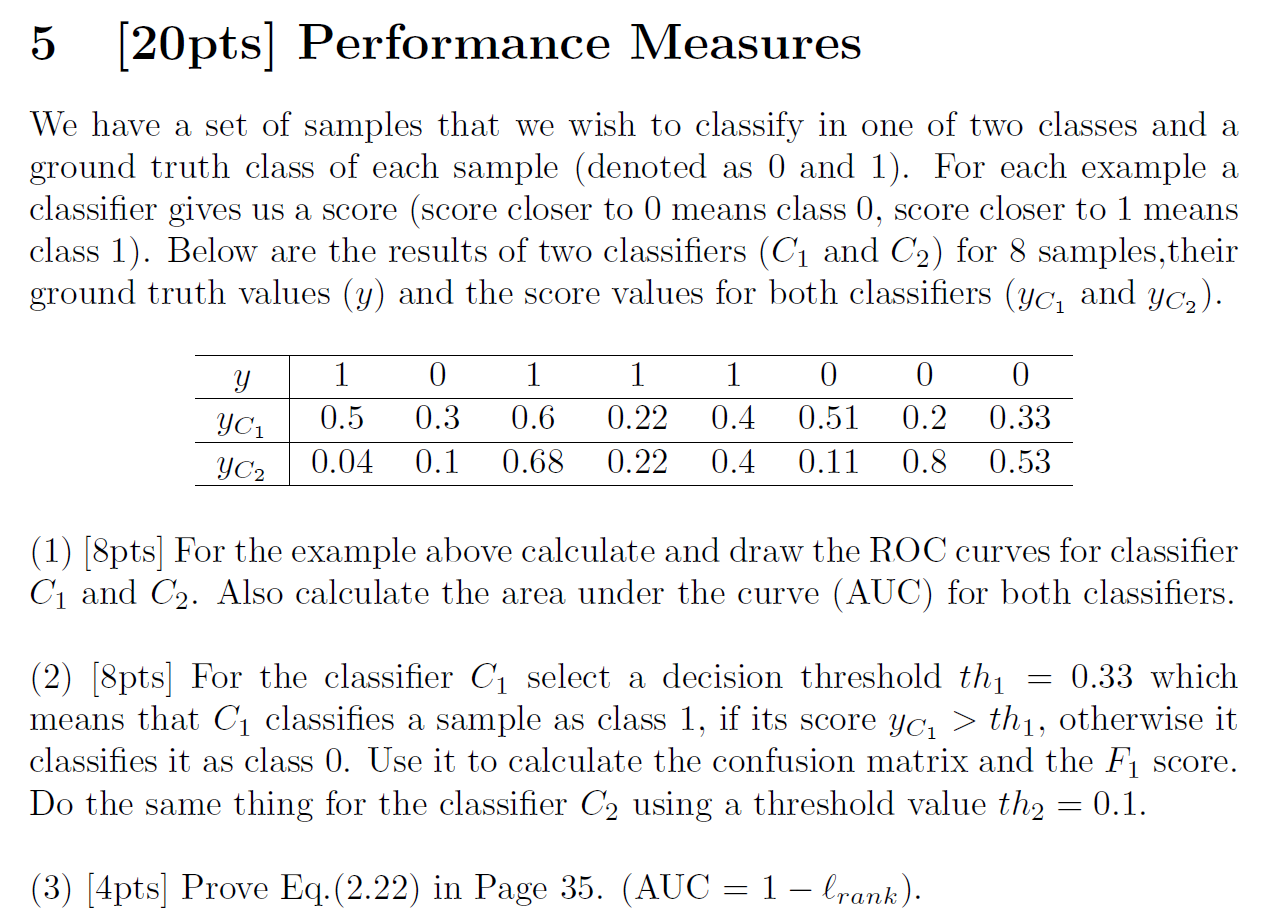
\includegraphics[scale=0.3]{5-p.png}

%\end{problem}
%\newpage
%\begin{solution}
   
%\end{solution}





%\begin{problem}[ML problem 6]
	
%\end{problem}
%\begin{solution}
    
%\end{solution}
%%%%%%%%%%%%%%%%%%%%%%%%%%%%%%%%%%%%%%%%%%%%%%%%%%%%%%%%%%%%%%%%
%                      Correction START!                       %
%%%%%%%%%%%%%%%%%%%%%%%%%%%%%%%%%%%%%%%%%%%%%%%%%%%%%%%%%%%%%%%%
%\begincorrection
%%%%%%%%%%%%%%%%%%%%
%\begin{problem}[]

%\end{problem}

%\begin{cause}
%
%\end{cause}

%\begin{revision}

%\end{revision}
%%%%%%%%%%%%%%%%%%%%
%\newpage
%%%%%%%%%%%%%%%%%%%%





%%%%%%%%%%%%%%%%%%%%%%%%%%%%%%%%%%%%%%%%%%%%%%%%%%%%%%%%%%%%%%%%
%                       Feedback START!                        %
%%%%%%%%%%%%%%%%%%%%%%%%%%%%%%%%%%%%%%%%%%%%%%%%%%%%%%%%%%%%%%%%
%\beginfb
%\begin{itemize}
%
%\end{itemize}





%%%%%%%%%%%%%%%%%%%%%%%%%%%%%%%%%%%%%%%%%%%%%%%%%%%%%%%%%%%%%%%%
%                        Homework END!                         %
%%%%%%%%%%%%%%%%%%%%%%%%%%%%%%%%%%%%%%%%%%%%%%%%%%%%%%%%%%%%%%%%
\end{document}
